% !TeX program = xelatex
\documentclass{article}
\usepackage{npu-report-style}
\usepackage{enumerate}

% 显示参考文献、引用超链接
\usepackage[breaklinks,colorlinks,linkcolor=black,citecolor=black,urlcolor=black]{hyperref}
% 关闭参考文献、引用超链接
%\usepackage[pagebackref=false, colorlinks, bookmarks=false ]{hyperref}

\usepackage{graphicx, subfig, epstopdf, amsmath, booktabs, paralist, float, caption, xfrac, enumitem, array, multirow, cite}

%\usepackage{graphicx, subfig, epstopdf, amsmath, booktabs, paralist, float, caption, xfrac, enumitem, array, multirow}

%\usepackage{subfigure}
\usepackage{subfloat}

\usepackage[heading=true]{ctex}

\usepackage{zhnumber} % change section number to chinese
\renewcommand\thesection{\zhnum{section}}
\renewcommand \thesubsection {\arabic{section}}
%\renewcommand \thesubsection {\arabic{subsection}}

%\usepackage{bibspacing}
%\setlength{\bibspacing}{\baselineskip}

\usepackage{url}
%\usepackage{cite}
% comma: 用逗号分隔多个引用; square:使用方括号; super:引用是上角标形式
\usepackage[square,sort,comma,numbers]{natbib}

%调整参考文献之间的距离(类似行距)
%\setlength{\bibsep}{9pt}

%加入下面这一行,非常灵活。 其中第一个参数是字体大小, 第二个参数是行距大小。自己可以视情况调整。
\def\bibfont{\fontsize{10.5pt}{12}\selectfont}


%\usepackage{natbibspacing}

%\usepackage{subfigure}
\usepackage{titlesec}
%\titleformat{\section}{\Large\bfseries}{\thesection、}{0em}{}
%\titleformat{\section}{\heiti\Large}{\thesection、}{0em}{}
%\titleformat{\subsubsection}{\kaishu\bfseries}{\thesection}{0em}{}

\titleformat{\section}{\heiti\zihao{-4}}{\thesection、}{0em}{}
\titleformat{\subsubsection}{\kaishu\bfseries\zihao{-4}}{\thesection}{0em}{}


%anonymous_review
%\def\anonymous{yes}

%\usepackage[heading=true]{ctex}

%\usepackage{gbt7714}

%\renewcommand{\bibname}{Reference}

\usepackage{caption}
\DeclareCaptionLabelSeparator{twospace}{\ ~}   %这三条语句即可
\captionsetup[figure]{labelsep=period,name={\kaishu 图}}
%\captionsetup{labelsep=period}
%\captionsetup[figure]{name={Fig.},labelsep=period} 
%space去掉点
%period加点
%不加space、period这两个就是冒号

% \newitemsep
% 下划线
\makeatletter
\newcommand\dlmu@underline[2][6cm]{%
	\hskip1pt\underline{\hb@xt@ #1{\hss#2\hss}}\hskip3pt}
\let\coverunderline\dlmu@underline
\makeatother


\ifx\anonymous\undefined
\def\author{张三}
\def\school{“卡脖子技术”研究院}
\def\mymajor{看文献找规律}
\def\idnumber{1024}
\def\supervisedsir{自学成才}
\def\anonymousSupervisedsir{}
\def\sirposition{\  教授}
\def\authorEnglishName{\textbf{S. Zhang}$^*$}
\def\supervisedsirEnglishName{\textbf{Z. Xue}$^\dag$}
\def\labName{XXX实验室}
\def\subjectName{XXX}
\else
	\def\author{}
	\def\school{}
	\def\mymajor{}
	\def\idnumber{}
	\def\supervisedsir{}
	\def\sirposition{}
	\def\anonymousSupervisedsir{***}
	\def\authorEnglishName{*}
	\def\supervisedsirEnglishName{\dag}
	\def\labName{***}
	\def\subjectName{***}
\fi

%\renewcommand\figureautorefname{图}		% 重新定义引用图标
%\renewcommand\tableautorefname{表}		% 重新定义应用表格
%\def\equationautorefname{式}				% 重新定义公式

% 设置 `论文题目' 
\nputitle{基于导师喜好的博士研究生学位论文命名方法关键技术研究}

\npunumber{\idnumber}
\npuschool{\school}
\npumajor{\mymajor}
\npuname{\author}
\npudegree{博士}
\npusupervisor{ \supervisedsir \sirposition}
\nputype{全日制学术型}
\npudate{\today}

% 博士
\npucheckphdtrue
% 第一次
\npucheckfirsttrue
%\npuchecksecondtrue

%% 设置 `论文类型': 取消或添加注释即可勾选相应类型
%\npucheckbasetrue   	%  基础研究
\npucheckapplytrue     	%  应用研究
%\npucheckenginetrue   	%  工程技术
%\npucheckoveralltrue   %  跨学科研究

\begin{document}
\section{学位论文研究依据}
\noindent{\zihao{-4}\kaishu 学位论文的选题依据和研究意义,国内外研究现状和发展态势,主要参考文献,以及已有的工作积累和研究成果。}
\subsubsection*{1.1选题背景和研究意义}
西北工业大学(Northwestern Polytechnical University)\ref{Fig. 1},简称“西工大”,位于陕西省西安市,是中华人民共和国工业和信息化部直属,中国唯一一所以同时发展航空、航天、航海工程教育和科学研究为特色的全国重点大学,位列国家“双一流”、“985工程”、“211工程”;入选“2011计划”、“111计划”、卓越工程师教育培养计划、国家大学生创新性实验计划、新工科研究与实践项目、国家建设高水平大学公派研究生项目、中国政府奖学金来华留学生接收院校;卓越大学联盟、中俄工科大学联盟、中俄交通大学联盟、中英大学工程教育与研究联盟、“一带一路”航天创新联盟、全国高等军工院校课程思政联盟成员,学位授权自主审核单位,欧盟QB50项目亚洲区唯一发起单位与亚洲区总协调单位。 

\begin{figure}[h!]
	\centering
	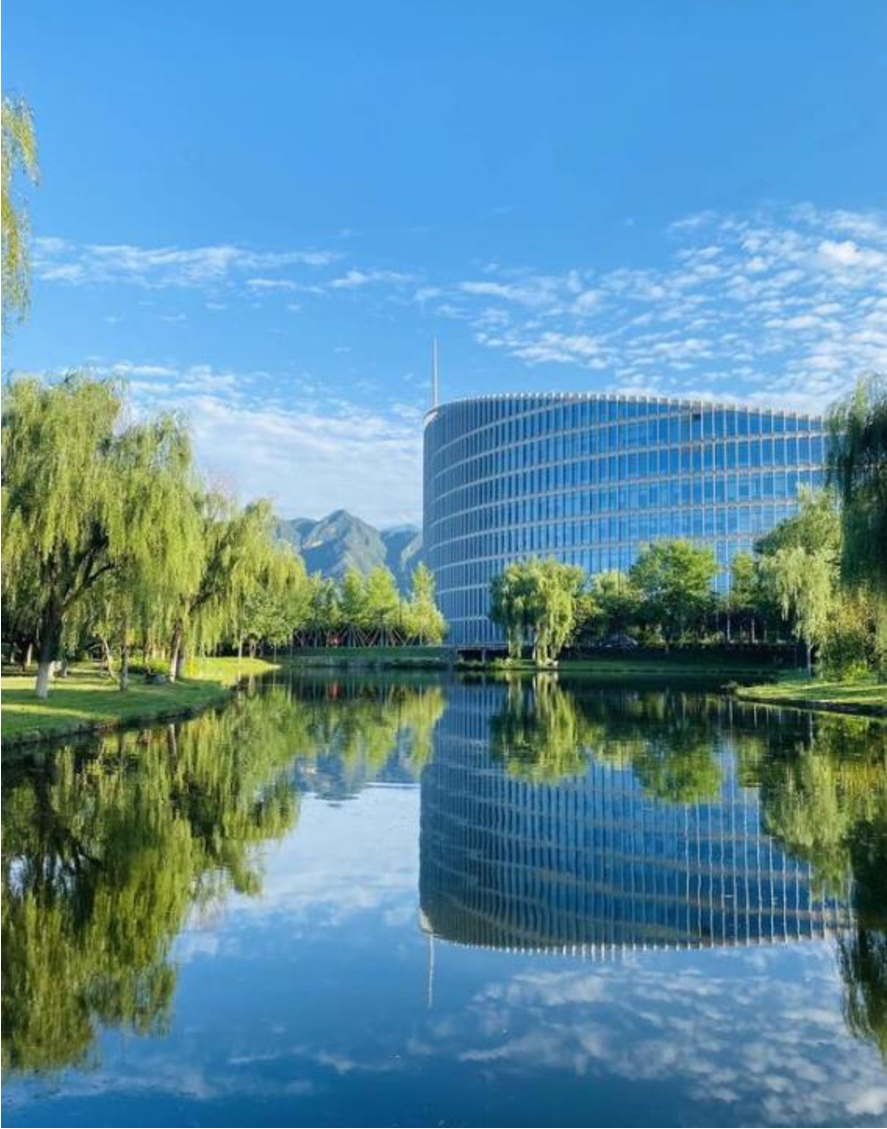
\includegraphics[width=0.5\textwidth]{figure/fig_1.pdf}
	\caption{\kaishu 西北工业大学}
	\label{Fig. 1}
\end{figure}
\vspace{-0.2cm}


1938年国立北洋工学院、国立北平大学工学院、国立东北大学工学院、私立焦作工学院在陕西汉中组建国立西北工学院;1946年迁至咸阳,1950年更名为西北工学院;1952年交通大学、浙江大学、南京大学的航空工程系在南京组建华东航空学院;1956年迁至西安,更名为西安航空学院;1957年,西北工学院与西安航空学院合并组建西北工业大学;1970年,原中国人民解放军军事工程学院航空工程系整体并入。

截至2021年11月,学校友谊、长安及江苏太仓三个校区占地面积7100多亩,下设27个学院、74个本科专业;拥有21个博士后流动站、25个一级学科博士点、38个一级学科硕士点;教职工4300余人,全职院士7人,在校生3.6万余人\cite{nwpu2020,da2019survey}。




%\vspace{-0.2cm}
\subsubsection*{1.2国内外研究现状}





%\vspace{0.5cm}
\subsubsection*{1.2.1 XXXXXX}

\begin{equation}
	\left \langle N,S,\left \{ A_{i}  \right \}_{i\in N},P,\left \{ r_{i}  \right \}_{i\in N},\gamma    \right \rangle \tag{1-1}
	\label{Equ.1}
\end{equation}




\subsubsection*{1.3存在问题及展望}

\begin{enumerate}
	\item[(1)] 111111
	\item[(2)] 222222
	\item[(3)] 333333
\end{enumerate}


\subsubsection*{1.4已有工作积累与研究成果}
	

\newpage
\bibliographystyle{nputhesis}          % 参考文献格式
\bibliography{reference}      % expects file "reference.bib
\newpage


\newpage
\section{学位论文研究内容}
\noindent{\kaishu 学位论文的研究目标、研究内容及拟解决的关键性问题(可续页)}
\subsubsection*{2.1论文的研究目标}

\subsubsection*{2.2论文的拟研究内容}
	
\subsubsection*{2.3拟解决的关键性问题}




\newpage
\section{学位论文研究计划及预期目标}
%\subsection*{1. 拟采取的主要理论、研究方法、技术路线和实施方案(可续页)}
\subsection*{\kaishu{3.1 拟采取的主要理论、研究方法、技术路线和实施方案}}


\newpage
%\subsection*{2. 研究计划可行性,研究条件落实情况,可能存在的问题及解决办法(可续页)}
\subsection*{\kaishu{3.2 研究计划可行性,研究条件落实情况,可能存在的问题及解决办法(可续页)}}


%\subsubsection*{3.2.2 可能存在的问题与解决方法}



\newpage
\subsection*{\kaishu{3.3 研究计划及预期成果}}


\begin{table}[h]
	\centering
	\renewcommand\arraystretch{1.5}
	
    \hrule height0pt \vfill
	\newlength{\tablesep}
	\setlength{\tablesep}{5pt}
	\newcolumntype{C}{>{\hfil}X<{\hfil}}
	\noindent\hskip-\npusep
	\begin{tabularx}{\npuwidth}{>{\centering}c|c|C}\hline
		\multirow{8}*{\parbox{0.05\npuwidth}{\centering  研\\究\\计\\划}}  & 起止年月 & 完成内容 
	\\ \cline{2-3} & 2020.03$ \sim $2020.12 & 西北工业大学(简称西工大)坐落于陕西西安。
	\\ \cline{2-3} & 2021.01$ \sim $2021.12 & 西北工业大学(简称西工大)坐落于陕西西安。
    \\ \cline{2-3} & 2022.01$ \sim $2022.06 & 西北工业大学(简称西工大)坐落于陕西西安,撰写小论文 1$ \sim $2 篇。
    \\ \cline{2-3} & 2022.07$ \sim $2022.12 & 西北工业大学(简称西工大)坐落于陕西西安,撰写小论文 1$ \sim $2 篇。
    \\ \cline{2-3} & 2023.01$ \sim $2023.06 & 西北工业大学(简称西工大)坐落于陕西西安,撰写小论文 1$ \sim $2 篇。
    \\ \cline{2-3} & 2023.07$ \sim $2023.12 & 西北工业大学(简称西工大)坐落于陕西西安,撰写小论文 1 篇。
    \\ \cline{2-3} & 2024.01$ \sim $2024.06 & 总结研究成果,完成博士学位论文撰写及答辩。
	\\ \hline
  \end{tabularx}
		
\end{table}



\noindent{\kaishu{预期创新点及成果形式}}





	


\end{document}